\scanpage{78}
$f$. For instance, using Chow's lemma and the Main existence theorem in my first talk on Picard schemes, one gets:

\uline{Corollary} 2\quad Assume $X/S$ proper satisfies the condition: \deleted{\unsure{a') for every}} \deleted{\unsure{any $X'$}\illegible{2} for} a') for every $X'$ finite over $X$, there \unsure{exists} a non empty open subset $S_1$ of $S$ such that \inserted{\handwritten{problem A for}} $X'\handwritten{\unsure{\mid|/}}S_1$ has allways solution \deleted{for problems A and B} (this condition is satisfied if $X/S$ is projective). Then \deleted{there exists} provided we replace $S$ by a suitable $S_1$ non empty and open, $\underline{\mathrm{Pic}}_{X/S}$ exists, is separated, its connected components are of finite type over $S$.

N.B. The proof does not give any evidence towards the fact that in the theorem, one could replace ``quasi-affine'' by ``affine'' . This is true however over a \unsure{fiéèd|fièèd|field}, because a quasi-affine algebraic group is affine ! It would be interesting to have a couterexample, say,over a \deleted{valuation} ring of dimension $1$ such as $k\handwritten{[}t\handwritten{]}$, $X$ and $X'$ \inserted{projective and} 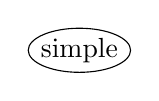
\begin{tikzpicture}[baseline=(w.base)]\node[inner sep=0pt] (w) {simple};\handwritten{\draw (w.center) ellipse (0.65cm and 0.28cm);}\end{tikzpicture}\margin{\handwritten{\figure{
\begin{tikzpicture}\draw (0,0) ellipse (0.25cm and 0.18cm);\end{tikzpicture}}impossible if\\$X$ smooth!}} over $S$ and $X'\handwritten{\to}X$ birational,orr alternatively, \deleted{\unsure{if $X'$ finite}} $X$ and $X'$ projective and normal over $S$, and $f:X'\handwritten{\to}X$ finite. A counterexample in the latter case would of course provide a counterexample to the effectivity problem\deleted{\unsure{s}} \inserted{for a finite morphism} raised in my first talk on descent \dots

``Problem A'' is the following: given $X/S$ and \deleted{any} Module $F$ on $X$, to represent the functor on the category of $S$-preschemes taking any $S'/S$ into \deleted{the empty or} into a one-element \inserted{or into the empty} set; according as to whether $F'$ on $X'/S'$ is flat with respect to $S'$\inserted{\handwritten{or not}}, where $X'=X\mathbin{x}_S S'$, $F'=F\unsure{2|x|\otimes}_S S'$. Given $X/S$, we say that ``Problem A \inserted{\handwritten{for $X/S$}} has always a solution'' if for every coherent $F'$ on \deleted{\unsure{$X$}}\inserted{\handwritten{some $X'/S'$}}, the previous functor \inserted{\handwritten{on $(\mathrm{Sch})/S'$}} is representable by a \inserted{$S\handwritten{'}$\handwritten{-}}scheme of finite type. The main step in my proof of existence of Hilbert schemes shows that this condition is satisfied when $X/S$ is projective,
% archive sheet number: 77
